\documentclass[useAMS,usenatbib,referee]{biom}

\usepackage{amsmath}
\usepackage[figuresright]{rotating}

\graphicspath{{include/}}

%%%%% PLACE YOUR OWN MACROS HERE %%%%%

\def\bSig\mathbf{\Sigma}
\newcommand{\VS}{V\&S}
\newcommand{\tr}{\mbox{tr}}



\title{Empirical Bayes analysis for detection of gene heterosis in RNAseq data}

\author{Jarad Niemi$^*$\email{niemi@iastate.edu}, 
Eric Mittman, 
Will Landau, and 
Dan Nettleton \\
Department of Statistics, Iowa State University, Ames, Iowa, U.S.A.}

\begin{document}

\date{{\it Received December} 2014} 

\pagerange{\pageref{firstpage}--\pageref{lastpage}} 
\volume{VV}
\pubyear{YYYY}
\artmonth{Month}
\doi{x}

\label{firstpage}

%  put the summary for your paper here

\begin{abstract}
This is the summary for this paper.
\end{abstract}

\begin{keywords}
Empirical Bayes; Gene expression; Heterosis; Hierarchical model; Negative binomial; RNAseq.
\end{keywords}

\maketitle

%  A maximum of six (6) tables or figures combined is often required.''

\section{Introduction}
\label{s:intro}

% Need to udpate as this is directly from Tieming's paper
Heterosis, or hybrid vigor, refers to the enhances phenotype of hybrid progeny relative to their inbred parents. Taking maize as an example, the offspring from crossing the inbred lines B73 and Mo17 are taller, mature faster, and produce greater yields than their parent lines \citep{hallauer1981quantitative, hallauer2010quantitative}. Since heterosis was scientifically documented by \cite{darwin1876effects}, it has been successfully manipulated to improve many species for food, feed, and fuel industries, such as rice \citep{yu1997importance}, alfalfa \citep{riday2002heterosis}, tomatoes \citep{krieger2010flowering}, and fish \citep{wohlfarth1993heterosis}. Despite the intensive study and successful utilization of heterosis, the basic genomic mechanisms remain unclear \citep{coors1999genetics, lippman2007heterosis}. Researchers speculate that gene-expression heterosis $-$ i.e, enhanced expression of one or more genes in the hybrid relative to the inbred parents $-$ could be among the mechanisms responsible for the phenotypic heterosis \citep{swanson2006all, springer2007allelic}.

% WML: Since you mainly talk about phenotypic heterosis, I added a little clarification about gene-expression heterosis. However, the reader will still be mostly focused on phenotypic heterosis, and more may need to be done to refocus on the transcriptome. Do we have good real-world examples of heterosis in the expression important or interesting genes? This may be a good question for Dan.

Recently \citep{ji2014estimation} provided an approach to assess heterosis using micro-array data using a hierarchical model for the ...

%\section{Heterosis}
%\label{s:heterosis}

% Well before heterosis was scientifically described by , humans had been using heterosis for various practical purposes. Within the last century, heterosis has been used to improve many species for food, feed, and fuel industries. A few relatively recent examples include rice , alfalfa , tomatoes . Despite the intensive study and successful utilization of heterosis, the basic genomic mechanisms responsible for heterosis remain unclear .
% 
% \cite{shull1952beginnings} coined the term heterosis and defined it as 
% \begin{quote}
% the interpretation of increased vigor, size, fruitfulness, speed of development, resistance to disease and to insect pests, or to climatic rigors of any kind, manifested by crossbred organisms as compared with corresponding inbreds, as the specific results of unlikeness in the constitutions of the uniting parental gametes. 
% \end{quote}
% 
% For example, the maize hybrid produced from a cross of parental inbred lines B73 and Mo17 is larger in size, has lower maturation time, and has higher grain yield than both of its parents \cite{hallauer2010quantitative}. Data from \citep{paschold2012complementation}
% 
% \citep{ji2014estimation}


\section{Empirical Bayes identification of gene heterosis from RNAseq counts}
\label{s:method}

An RNAseq experiment to identify genes demonstrating heterosis consists of three genetic varieties: two parental varieties (P1 and P2) and a cross between these two varieties called the hybrid (H). For each variety, replicate RNA samples are isolated and assessed for quality. cDNA libraries, i.e. short cDNA fragments, are constructed and next generation sequencing technology is used to determine the \emph{reads}, i.e. nucleotide sequences in the cDNA libraries. These reads are processed using bioinformatic algorithms to match the reads to genes, or specific gene transcripts, exons, microRNAs, etc. The result of matching reads to features are summarized by a gene $\times$ sample matrix of counts. For more details on RNAseq experiments see \cite{nettleton2014design} and for biological background on the details of these steps see \cite{paschold2012complementation}.

To identify genes displaying heterosis using RNAseq counts, we build a hierarchical model to borrow information on gene-variety means as well as overdispersion parameters, estimate the parameters using a empirical Bayes procedure implemented in the statistical software {\tt Stan}, and calculate empirical Bayes posterior probabilities for heterosis. 


\subsection{Hierarchical model for RNAseq counts}
\label{s:model}

Let $Y_{gvi}$ be the count for gene $g=1,\ldots,G$, variety $v=1,\ldots,V$, and replicate $i=1,\ldots,n_v$. As shown in equation \eqref{e:data}, we assume a negative binomial for the counts with a mean that depends on the gene-variety combination through $\mu_{gv}$ and the sequencing depth $c_{vi}$ and a gene-specific over-dispersion $\psi_g$. Here $NB(\eta,\psi)$ indicates a negative-binomial with expectation $\eta$ and variance $\eta+\psi\eta^2$ and $ind$ indicates the observations are conditionally independent.
\begin{equation} 
Y_{gvi} \stackrel{ind}{\sim} NB(e^{\mu_{gv}+\delta_{vi}},\psi_g) 
\label{e:data}
\end{equation}

A hierarchical model is constructed for the sequencing depth, overdispersion, and gene-variety parameters. The sample-specific sequencing depth terms are assumed to follow a normal distribution, i.e. $\delta_{vi} \stackrel{ind}{\sim} N(0,\tau_\delta^2)$. The logarithm of the gene-specific over-dispersion parameters and the gene-specific variety effects are assumed to have a joint normal distribution, i.e. 
$\theta_g = [\mu_g, \log(\psi_g)]^\top \stackrel{ind}{\sim} N\left(\eta, \Sigma\right)$
where $\mu_g = (\mu_{g1},\ldots,\mu_{gV})'$. We consider an \emph{independent} model where $\Sigma$ is diagonal with elements $\sigma_1^2,\ldots,\sigma_{V+1}^2$ and a \emph{covariance} model where we estimate all parameters in $\Sigma$. 

We assume improper uniform priors for $\eta$ and $\tau_\delta\stackrel{ind}{\sim} Ca^+(0,3)$ where 0 and 3 are the location and scale parameters of the untruncated distribution. In the independent model, we also $Ca^+(0,3)$ on the diagonal elements of $\Sigma$ while in the covariance model, we assume a conjugate, proper inverse Wishart with degrees of freedom $V+2$ and an identity scale matrix which results in marginally uniform correlations. 

\subsection{Empirical Bayes}
\label{s:ebayes}

The parameters from the model in Section \ref{s:model} can be group by gene-specific parameters $\theta = (\theta_1,\ldots,\theta_G)$, and hyperparameter $\phi = (\delta,\eta, \Sigma)$ where $\delta = (\delta_{11},\ldots,\delta_{Vn_V})$. We employ an optimization procedure to obtain the \emph{maximum a posteriori} (MAP) estimate for $\phi$, denoted $\hat{\phi}$, and then base gene-specific inference on the posterior conditional on this estimated hyperparameter. Conditional on the hyperparameters, the gene-specific parameters are conditionally independent as in equation \eqref{e:condind}. Thus, conditional posterior inference for the gene-specific parameters can be obtained independently and in parallel.
\begin{align}
p\left(\theta\left|y,\hat{\phi}\right.\right) 
%&= \prod_{g=1}^G p\left(\theta_g\left|y_g,\hat{\phi}\right.\right) = \prod_{g=1}^G p\left(y_g\left|\theta_g,\hat{\delta}\right.\right) p\left(\theta_g\left|\hat{\phi}\right.\right) \nonumber \\
&\propto \prod_{g=1}^G \left[ \prod_{v=1}^V \prod_{i=1}^{n_v} NB\left(y_{gvi}\left|e^{\mu_{gv}+\hat{\delta}_{vi}},\psi_g\right.\right) \right] N\left(\left.\left[\mu_g, \log(\psi_g) \right]^\top\right|\hat{\eta}, \hat{\Sigma} \right) 
\label{e:condind}
\end{align}


To perform the optimization, we use the statistical software {\tt Stan} \citep{stan-software:2014} run through the RStan interface \citep{rstan-software:2014} in R \citep{R2014}. The Stan software allows construction of general Bayesian models with the primary restriction that all unknown parameters must be continuous. Once a model is constructed, the software can be used to obtain MAP estimates \cite[Section 50.3,][]{stan-manual:2014} using the {\tt optimizing} function in RStan. We found it necessary to use the L-BFGS algorithm \cite[Section 55,][]{stan-manual:2014} presumably due to the large dimension of the optimization. The {\tt Stan} software can also be used to run a Markov chain Monte Carlo (MCMC) algorithm to obtain samples from the posterior using the {\tt sampling} function in RStan. By default, Stan uses a variant of Hamiltonion Monte Carlo \citep{neal2011mcmc} called the no-U-turn sampler \citep{hoffman2013no}. 

As we have not integrated out the gene-specific parameters when obtaining the MAP estimate, we actually receive a joint MAP estimate for $\theta$ and $\phi$. We explicitly use the MAP estimate for $\phi$ when obtaining empirical Bayes posterior samples for the gene-specific parameters as in equation \eqref{e:condind}. The MAP estimate for $\theta$ can also be used in this step as initial values for the MCMC. 

\subsection{Gene heterosis}
\label{s:gene_heterosis}

As defined in Section \ref{s:intro}, heterosis is increased (or decreased) phenotypic expression in a hybrid relative to its inbred parents. Thus, when attempting to identify heterosis, there are three varieties of interest, i.e. $V=3$. We let $v=1,2$ be the two parental varieties and $v=3$ be the hybrid. We define gene heterosis to be the differential expression of the hybrid relative to its parents. For a specific gene $g$, low-parent gene heteorisis (LPH) occurs when $\mu_{g3}< \min(\mu_{g1},\mu_{g2})$, mid-parent gene heterosis occurs when $\mu_{g1}\le \mu_{g3}\le \mu_{g2}$ if $\mu_{g1}\le \mu_{g2}$ (or $\mu_{g1}\ge \mu_{g3}\ge \mu_{g2}$ if $\mu_{g1}\ge \mu_{g2}$), and high-parent gene heterosis (HPH) occurs when $\max(\mu_{g1},\mu_{g2}) < \mu_{g3}$. For simplicity, we define \emph{extreme gene heterosis} (EH) which is the event of LPH or HPH. Of interest is to evaluate the hypotheses shown in equation \eqref{e:hypotheses} where $H_0$ indicates no EH and $H_1$ indicates EH. 
\begin{align}
\label{e:hypotheses}
H_{g0}:&\mu_{g1}\le \mu_{g3}\le \mu_{g2} \mbox{ or } \mu_{g1}\ge \mu_{g3}\ge \mu_{g2} \mbox{\ \ vs.\ \ } \nonumber \\
H_{g1}:&\mu_{g3}< \min(\mu_{g1},\mu_{g2}) \mbox{ or } \max(\mu_{g1},\mu_{g2}) < \mu_{g3}.
\end{align}
We evaluate these hypotheses based on empirical Bayes estimates of their posterior probability, e.g. 
\begin{align}
P\left(H_{g1}|y, \hat{\phi}_{MAP}\right) &= P\left(\left.\mu_{g3}< \min(\mu_{g1},\mu_{g2}) \mbox{ or } \max(\mu_{g1},\mu_{g2}) < \mu_{g3}\right| y, \hat{\phi}_{MAP}\right) \nonumber \\
&\approx \frac{1}{M} \sum_{m=1}^M \mathrm{I}\left(\mu_{g3}^{(m)}< \min\left(\mu_{g1}^{(m)},\mu_{g2}^{(m)}\right) \mbox{ or } \max\left(\mu_{g1}^{(m)},\mu_{g2}^{(m)}\right) < \mu_{g3}^{(m)}\right) \label{e:probs}
\end{align}
where $\mu_g^{(m)} = \left(\mu_{g1}^{(m)},\mu_{g2}^{(m)},\mu_{g3}^{(m)}\right)$ is the $m^{th}$ MCMC sample from the empirical Bayes posterior and $\mathrm{I}(A)$ is 1 if A is true and 0 otherwise. The set of probabilities $P\left(H_{g1}|y, \hat{\phi}_{MAP}\right)$ for $g=1,\ldots,G$ can be used to provide a list of genes sorted by the relative strength of evidence for extreme heterosis. This list can be used by geneticists to prioritize future experiments to understand the genetic mechanism for heterosis.  

\section{Simulation study based on maize experiment}
\label{s:simulation}

% \subsection{Coverage for our model}
% \input{../temp/analyze-heterosis/FIGURES/coverage}

To assess the efficacy of our method to identify genes demonstrating heterosis, we used a maize data set with parental varieties B73 and Mo17 and the hybrid variety (B73 $\times$ Mo17) \citep{paschold2012complementation}. We compared our method to approaches using the R packages {\tt edgeR}, {\tt baySeq}, and {\tt ShrinkBayes}.

\subsection{Constructing simulated data}
\label{s:sim_data}

Initially, the maize experiment had RNAseq counts for 39,656 genes and 4 replicates per variety. We eliminated low count genes by removing any gene with three or more zeros for any variety and genes whose mean count across the varieties was less than one, which resulted in 27,888 genes remaining.

To begin, we applied the {\tt edgeR} package from Bioconductor (citation needed) to the maize data to obtain sample-specific normalization factors, then gene-specific dispersions, and finally gene-variety-specific location parameters. We treated these parameters as the truth for the simulation study: i.e. a gene with $\mu_{g3} < \min(\mu_{g1}, \mu_{g2})$ was considered to have LPH, while a gene with $\max(\mu_{g1},\mu_{g2}) < \mu_{g3}$ was considered to have HPH. This technique ensured that our simulated datasets maintained the existing covariance structure among the gene-variety means of the original maize data.

Using these parameters and normalization factors, we simulated data according to the negative-binomial model in equation \eqref{e:data} independently for each gene. For each simulation, low count genes, i.e. those with three or more zeros in any variety or whose mean count across the varieties was less than one, were removed. A random set of 25,000 genes was retained from those with high enough counts. This simulation process was repeated 10 times for each of 4, 8, and 16 replicates per variety (reusing normalization factors when necessary).

\subsection{Alternative methods}
\label{s:alternative}

Existing RNAseq data analysis methods are not specifically designed to identify gene heterosis, but we adapted the approaches in {\tt edgeR}, {\tt baySeq}. and {\tt ShrinkBayes} to provide statistics to measure the strength of extreme heterosis of each gene.

{\tt edgeR} is designed to apply a negative binomial loglinear model to test for differential expression between any two varieties \citep{robinson2007moderated, robinson2010edgeR}, and we used this capability to construct a pseudo-probability of heterosis for each gene. We first computed the maximum likelihood estimates of the mean expression effects of all genes using {\tt edgeR}'s built-in Fisher scoring algorithm, and then we used the likelihood ratio test functionality to calculate two legitimate p-values for each gene: one for the null hypothesis that the hybrid's mean expression is the same as that of parent 1 and the second for the analogous test involving parent 2. For each gene, if the estimated mean expression level of the hybrid is not between the estimated mean expression levels of the parents, we set the pseudo-probability of heterosis to be one minus the p-value corresponding to the parent with estimated expression level closer to that of the hybrid. Otherwise, the pseudo-probability is zero.

The {\tt baySeq} approach allows for a wider range of hypotheses for each gene, including $H_1: \mu_{g1}=\mu_{g2}=\mu_{g3}$, $H_2: \mu_{g1}=\mu_{g2}$, $H_3: \mu_{g1}=\mu_{g3}$, $H_4: \mu_{g2}=\mu_{g3}$, and $H_5:$ all $\mu_g$'s are distinct \citep{hardcastle2010bayseq, hardcastle2012baySeq}. In a technique similar to our application of {\tt edgeR}, we used used the posterior probabilities of these hypotheses to construct a pseudo-probability of heterosis for each gene. We set this pseudo-probability to zero if the hybrid's maximum likelihood estimate of the mean expression level calculated with {\tt edgeR} is between those of the parents. Otherwise, the pseudo-probability is the sum of the posterior probabilities of $H_2$ and $H_5$. Note that $H_2$ and $H_5$ are the only hypotheses that allow for heterosis.

The {\tt ShrinkBayes} package implements fully Bayesian inference through integrated nested Laplace approximation (INLA) \citep{rue2009approximate,van2014shrinkbayes}. A limitation of INLA is that it only provides approximations to marginal posteriors for parameters or linear combinations of parameters rather than an approximation to the full posterior. Thus, we cannot directly estimate nonlinear quantities such as $P(\mu_{g3} < \min(\mu_{g1},\mu_{g2}))$. To circumvent this limitation, we reparameterized the independence model in Section \ref{s:model} using the approach in \cite{ji2014estimation}. 
Let $\gamma_g = (\mu_{g1}+\mu_{g2})/2$ be the parental log-mean, $\alpha_g = (\mu_{g2}-\mu_{g1})/2$ be the half parental difference, and $\zeta_g = \mu_{g3} - \gamma_g$ be the hybrid effect. After fitting the model with {\tt ShrinkBayes}, we constructed a pseudo-probability of heterosis for each gene. For gene $g$, we used the estimated posterior means $\hat{\zeta}_g$ and $\hat{\alpha}_g$ of $\zeta_g$ and $\alpha_g$, respectively, along with appropriate posterior probabilities $P(\cdot \mid y)$. Specifically, the pseudo-probability of heterosis for gene $g$ is zero if $|\hat{\zeta}_g| \le |\hat{\alpha}_g|$, $P(\zeta_g + \alpha_g > 0 |y)$ if $\hat{\zeta}_g > -\hat{\alpha}_g \ge 0$, $P(\zeta_g - \alpha_g > 0 |y)$ if $\hat{\zeta}_g > \hat{\alpha}_g \ge 0$, $P(\zeta_g - \alpha_g < 0 |y)$ if $\hat{\zeta}_g < \hat{\alpha}_g \le 0$, and $P(\zeta_g + \alpha_g < 0 |y)$ if $\hat{\zeta}_g < -\hat{\alpha}_g \le 0$.  

\subsection{Results}

For each of the methods above as well as the method described in Section \ref{s:gene_heterosis}, we sorted genes according to the plausibility of heterosis. From these sorted lists, we constructed receiver-operating characteristic (ROC) curves to evaluate the ability of these methods to identify genes with heterosis, as defined in Section \ref{s:sim_data}, \citep{landau2013dispersion}. A representative set of ROC curves is shown in Figure \ref{f:roc}. 
\begin{figure}[htbp]
\centerline{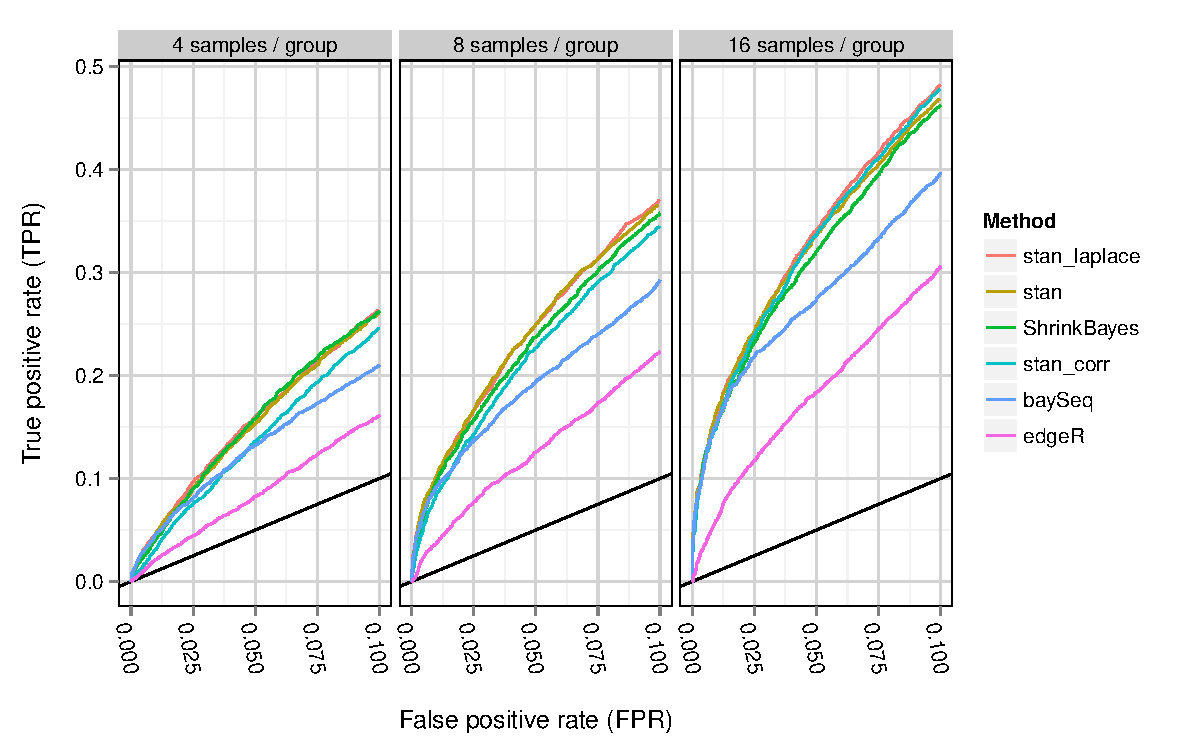
\includegraphics[width=\textwidth]{exampleROC0_1}}
\caption{Repersentative ROC curves for false positive rates below 0.1 for the approaches using {\tt edgeR}, {\tt baySeq},  and {\tt ShrinkBayes} described in Section \ref{s:alternative} and the method using {\tt RStan} assuming independence and with a covariance described in Section \ref{s:gene_heterosis}.}
\label{f:roc}
\end{figure}
For this simulation, we can see the approaches based on the model in Section \ref{s:model}, i.e. both RStan approaches and the ShrinkBayes approach, provide the best true positive rate for a given false positive rate. Also, as expected, as the sample size increases our ability to distinguish genes with heterosis from genes without improves.

Figure \ref{f:auc} provides the area under the ROC below a false positive rate of 0.1 across the 10 simulations for each of the 3 different sample sizes. 
\begin{figure}
\centerline{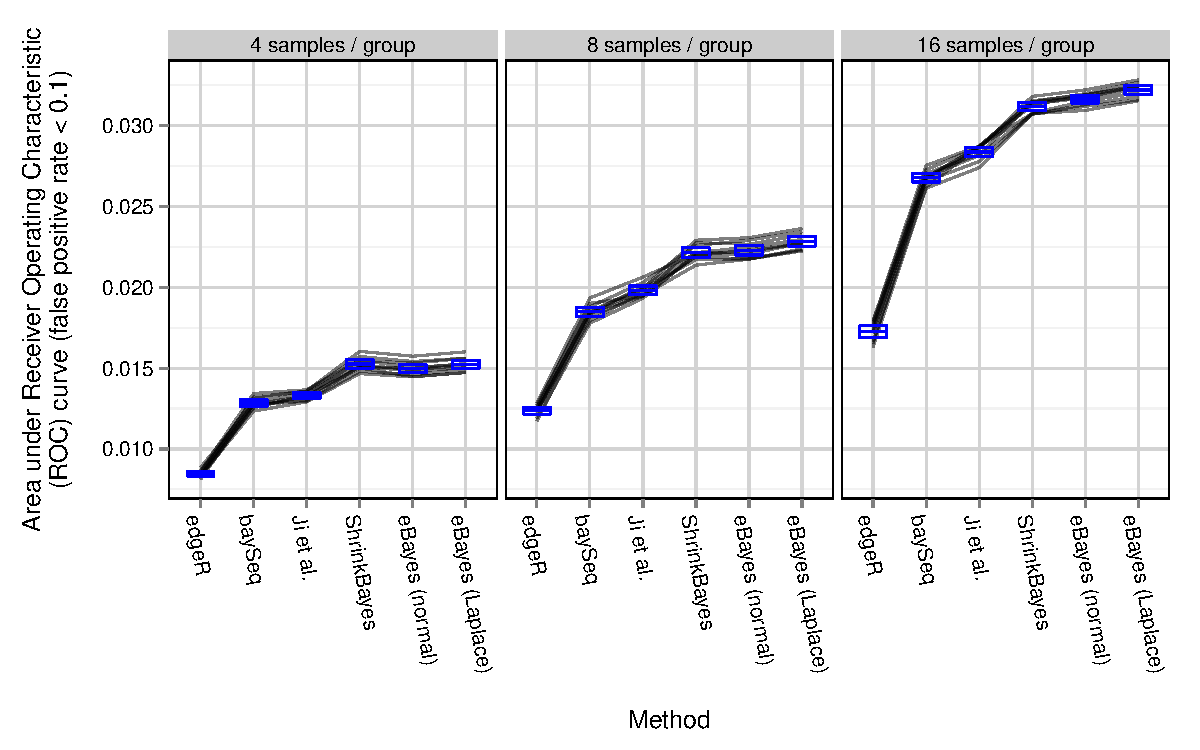
\includegraphics[width=\textwidth]{auc-facet-TRUE}}
\caption{Area under the ROC curves below a false positive rate of 0.1 for 3 different sample sizes for the approaches using {\tt edgeR}, {\tt baySeq},  and {\tt ShrinkBayes} described in Section \ref{s:alternative} and the method using {\tt RStan} assuming independence and with a covariance described in Section \ref{s:gene_heterosis}. Each line is a different simulation while the blue box indicates mean AUC and its standard error across the simulations.}
\label{f:auc}
\end{figure}
The pattern appears to hold with the {\tt RStan} and {\tt ShrinkBayes} approaches outperforming the other two. While there does not appear to be a significant difference between the independence model using RStan or ShrinkBayes, there does appear to be a significant decreased performance, at least for smaller sample sizes, when using the model where a covariance is estimated. 


\section{Heterosis in maize ??}
\label{s:corn}

We calculate an estimated effect size using the posterior means for the gene-specific parameters using the formula 
\[
\mbox{estimated effect size} = \left\{ 
\begin{array}{ll}
\hat{\mu}_{g3} - \min(\hat{\mu}_{g1},\hat{\mu}_{g2}) & \mbox{if } \hat{\mu}_{g3} < \min(\hat{\mu}_{g1},\hat{\mu}_{g2}) \\
\hat{\mu}_{g3} - \max(\hat{\mu}_{g1},\hat{\mu}_{g2}) & \mbox{if } \hat{\mu}_{g3} > \max(\hat{\mu}_{g1},\hat{\mu}_{g2}) \\
0 & \mbox{otherwise}.
\end{array} 
\right. 
\]
Figure \ref{f:volcano} provides a volcano plot to visualize the probability of heterosis versus estimated effect size. 

\begin{figure}
\centerline{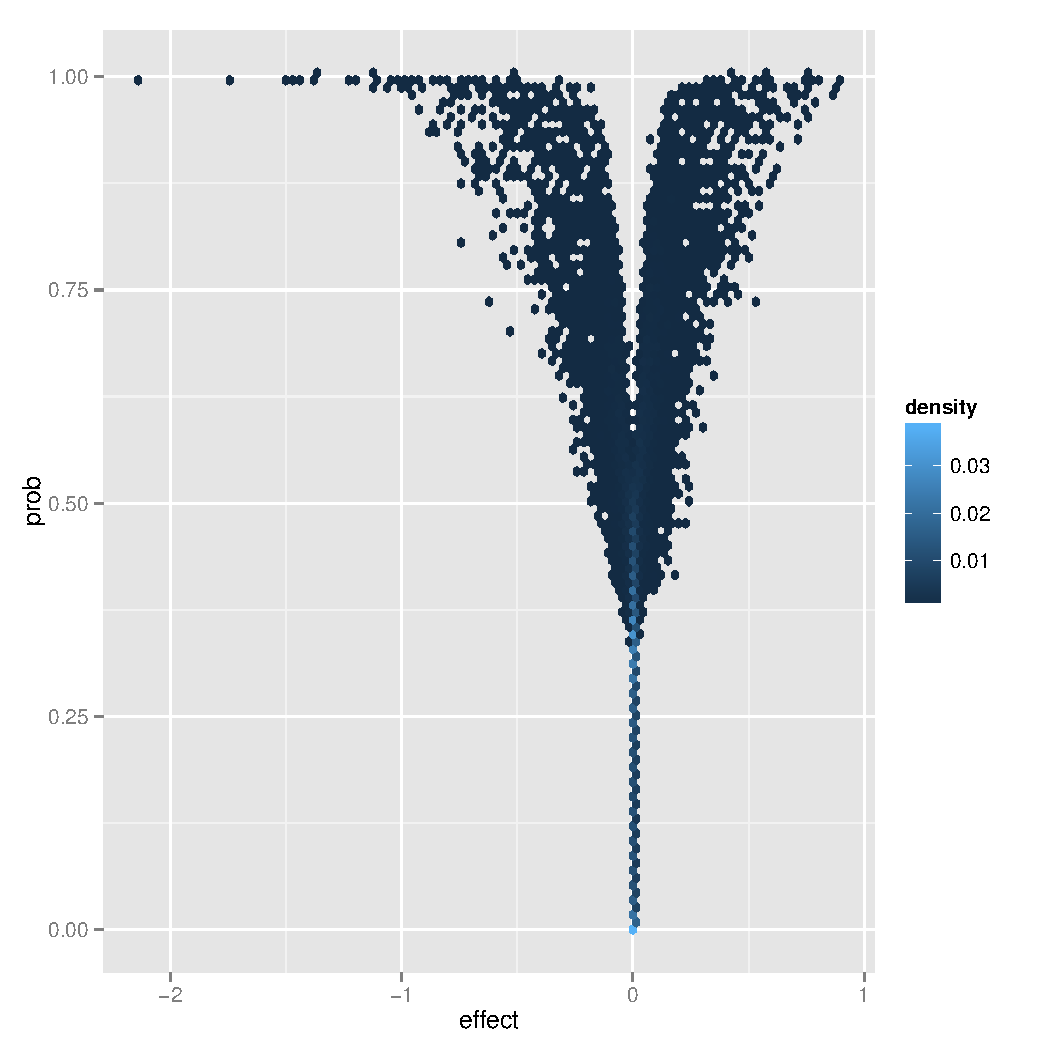
\includegraphics[width=\textwidth]{volcano}}
\caption{A two-dimensional histogram of the maximum of LPH and HPH probabilities versus estimated effect size, $\mu_{g3}-\max(\mu_{g1},\mu_{g3})$ if $P(HPH|y)>P(LPH|y)$ or $\mu_{g3}-\min(\mu_{g1},\mu_{g2})$ if $P(HPH|y)<P(LPH|y)$ for the B73 $\times$ Mo17 maize experiment.}
\label{f:volcano}
\end{figure}

\begin{figure}
\centerline{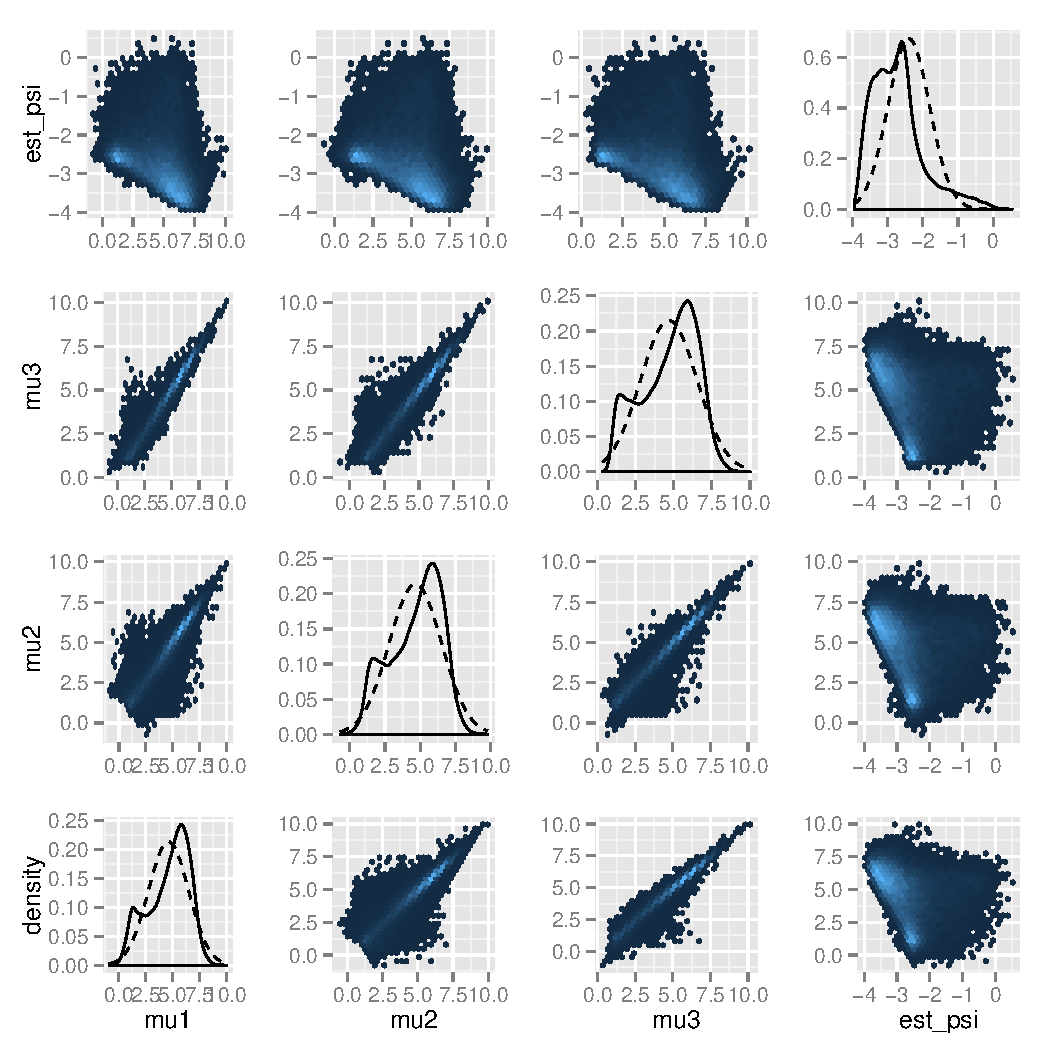
\includegraphics[width=\textwidth]{normality}}
\caption{One and two-dimensional histograms for gene-specific parameters from a single MCMC iteration, $\theta_g^{(m)}$,  for the B73 $\times$ Mo17 maize experiment. For reference, the one dimensional histograms have the marginal probability density functions from $N(\hat{\eta},\hat{\Sigma})$.}
\label{f:normality}
\end{figure}



\section{Discussion}
\label{s:discuss}

Put your final comments here. 



\backmatter %  Please keep this command in your document in this position 



\section*{Acknowledgements}

The authors thank Andrew Lithio for help implementing our model in {\tt ShrinkBayes}. Research reported in this publication was supported by National Institute of General Medical Sciences of the National Institutes of Health under award number R01GM109458. The content is solely the responsibility of the authors and does not necessarily represent the official views of the National Institutes of Health.

%  If your paper refers to supplementary web material, then you MUST
%  include this section!!  See Instructions for Authors at the journal
%  website http://www.biometrics.tibs.org

\section*{Supplementary Materials}


\bibliography{jarad}
\bibliographystyle{biom}

\appendix

%  To get the journal style of heading for an appendix, mimic the following.

\section{}

\label{lastpage}

\end{document}
